\chapter{Diffusion Models for Surrogate Simulation}

Developing probabilistic generative models for physics data is a demanding yet fruitful task.
A major challenge posed by increasing collider experiment data is the computational resources required for detailed simulations.
Fast surrogate models can reduce the computational cost of event and detector simulation, can be used for template-based anomaly detection, or the inverse problem of unfolding.

One of the early objectives of this thesis was to develop a generative model specifically for collider data.
Unlike the data used in CV, it is inherently point-like, and unlike the data used in NLP, it is unordered and continuous.
These characteristics make physics data well suited to graphical representations, hence the success of GNNs models in jet tagging, as discussed in \Cref{ch:spice}.
Set generation methods, typically benchmarked on the ShapeNet dataset~\cite{ShapeNet}, provided a natural starting point for this work.

Other research groups had explored GNNs trained as GANs~\cite{MPGAN}, achieving some success but also encountered the typical drawbacks of GANs as detailed in \Cref{ch:generative_models}.
Our initial efforts focused on developing a graph-based VAE~\cite{SetVAE}, using a GNN decoder to transform pure noise into a reconstructed point cloud conditioned on the latent space.
While this approach worked on ShapeNet, it failed to generate high-quality samples of particle physics data.
The primary issue was identifying a suitable permutation-invariant loss term for reconstruction. Various attempts were made, including modifications to Sinkhorn~\cite{Sinkhorn}, Chamfer, and optimal transport losses, as well as physically motivated metrics specific to collider data~\cite{MetricSpaceCollider}, all yielding suboptimal results.

As diffusion models started to gain prominence, a realization was made that these models do not require permutation invariant losses as the training objective for diffusion models is denoising rather than generation.
This task is already permutation equivariant and thus could be achieved even using MSE, leading to the development of the first diffusion model for generating particle-type data.

This chapter summarizes a collection of work done to develop models for the conditional generation of set data, including particle physics jets~\cite{PCJedi, EpicJedi, PCDroid} and full events~\cite{PIPPIN}.
It also covers the use of these models for template-based anomaly detection~\cite{Drapes, RadOT}.

\section{\pcjedi}

A practical initial task for developing a generative model for collider data is generating individual particle physics jets.
These collimated showers of hadrons produce electrically charged and neutral particles within a cone originating from the interaction point.
Jet formation involves transitioning from colour-charged partons, explainable via perturbative QCD, to a collection of colour-singlet hadrons, leptons, and photons interacting with the detector material.
While both regimes are well understood, the transition between them is not and continues to be a focal point of ongoing research.

Parton showers are iteratively constructed using a simple Markovian algorithm that stochastically transitions an $n$-parton state to an $(n+1)$-parton state.
Eventually, these are mapped to colour-singlet hadrons in a process called hadronization.
These final state particles are also called the jet constituents or the particle cloud.
This chain of events is simulated using dedicated generators such as \pythia~\cite{Pythia8}, \sherpa~\cite{Sherpa}, and \herwig~\cite{Herwig}.
This is typically followed by interactions with detector material performed using \geant~\cite{Geant4}.
The high multiplicity of particles, the stochastic nature of showers, and the complex detector response make jets computationally expensive to simulate.

Fast parametric simulation tools already exist, such as \delphes~\cite{Delphes}, which replaces the computationally expensive \geant in situations where computational resources are limited and the incurring a loss of detail is acceptable.
Therefore, it is not a stretch to use a deep generative model for specific tasks in the simulation pipeline.
Alternatively, the model could jump straight to simulating the detector response from the initial parton kinematics.

Our first attempt was to develop a model to conditionally generate the particle cloud, bypassing the showering, fragmentation, and hadronization steps.
We developed this model for large-radius jets, which have complex substructure and are used in many analyses at the LHC.
As we were performing a set generation task, we required the model to be based on a GNN.
Our first model for this task was called \pcjedi~\cite{PCJedi} (Particle Cloud Jet Diffusion)\footnote{Code for this project is publicly available~\cite{PCJediCode}}.

\subsection{Diffusion Schedule}

\pcjedi was developed using the score matching diffusion framework from~\textcite{ScoreBasedGenerativeModeling} which is covered in \Cref{sec:score_based}.
We chose to use SM-TI schedule with hyperparameters $\sigma_\text{max}<1$ and $\sigma_\text{min}>0$, giving the following expressions for the signal and noise levels,
\begin{align}
    \lambda_a & = \arccos(\sigma_\text{max}),                           \\
    \lambda_b & = \arccos(\sigma_\text{min}),                           \\
    s(t)      & = \cos\bigl(\lambda_a + t(\lambda_b - \lambda_a)\bigr), \\
    \sigma(t) & = \sin\bigl(\lambda_a + t(\lambda_b - \lambda_a)\bigr).
\end{align}
Following the derivation in \Cref{sec:score_based}, this results in the reverse SDE of the form,
\begin{equation}
    \label{eq:jedi_reverse_vp_sde}
    \diff\x_t = f(t) \left[ \x_t + 2 \score \right] \diff t + \sqrt{2 f(t)} \diff \bar\w_t,
\end{equation}
and the probability flow ODE,
\begin{equation}
    \label{eq:jedi_vp_ode}
    \diff \x_t = f(t) \left[ \x_t + \score \right] \diff t.
\end{equation}
Here $f(t)$ is related to the signal rate via,
\begin{equation}
    s(t) = \exp\left(\int_0^t f(s) \diff s\right),
\end{equation}
and solving this equation yields
\begin{equation}
    f(t) = (\lambda_b - \lambda_a) \tan\bigl(\lambda_a + t(\lambda_b - \lambda_a)\bigr).
\end{equation}

This task was framed using the standard SM objective, where a neural network is trained to predict the noise that was used to corrupt some data sample from \Cref{eq:noise_loss}.
This is extended for conditional generation based on context variable $\con$ and a hybrid loss term to give the training objective,
\begin{equation}
    \label{eq:training_objective}
    \mathcal{L}(\theta) =
    \E_{t\sim \mathcal{U}(0, 1)}
    \E_{\x_0, \con \sim \mathcal{D}},
    \E_{\z \sim \normal}
    \left(1 + \alpha \frac{4f(t)^2}{\sigma(t)^2}\right)
    \| \hat\e_\theta (\x_t, t, \con) - \e \|^2.
\end{equation}
The coefficient $\sfrac{4f(t)^2}{\sigma(t)^2}$ ensures that training corresponds to a maximum likelihood objective.
However, this can lead to unstable training, so many models in CV use the simple objective with no extra coefficient in front of the loss.
We use hyperparameter $\alpha$ to that controls the relative weight of these two tasks~\cite{ImprovedDenoisingDiffusion}.

\subsection{Data}
\label{sec:jetgen_data}

We used the open dataset JetNet30~\cite{MPGAN} in these experiments.
Proton-proton collision events were simulated with a centre of mass energy $13~\TeV$ at leading order using \madgraph~\cite{MadGraph} and the \textsc{NNPDF2.3LO}~\cite{PDF2.3} set of parton distribution functions.
The transverse momenta of the partons and bosons were generated with $\pt \approx 1~\TeV$.
Showering was performed using \pythia 8.212~\cite{Pythia8} with the Monash tune~\cite{Monash}.
Jets were clustered using the anti-$k_T$ algorithm~\cite{AntiKt} with a distance parameter $R=0.8$ using \fastjet~\cite{FastJet} and were required to have reconstructed $0.8 < \pt < 1.6~\TeV$.
No detector simulation was performed.
Five classes of jets were simulated based on the initiating particle: $q$ - light quark; $g$ - gluon; $t$ - top quark; $W$ - $W$ boson; $Z$ - $Z$ bosons.
Around 170k jets were produced for each class, with 50k reserved for evaluation; however, for \pcjedi, we only used the gluon and top quark datasets.

Jets were described in the dataset by their net kinematics, such as \mjet and \ptjet, as well as a list of the leading 30 constituents in \pt.
No constituent identification is provided, and each is effectively massless, thereby described solely by their three momenta.
Limiting the particle cloud to only 30 constituents meant the saved jet kinematics were not the same as net kinematics of the truncated particle cloud, which we identify as \mpc and \ptpc.
This distinction is important when evaluating the model.

\subsubsection{Input and Conditional Features}

The task of the model was to generate the properties of the particle cloud given requested cloud properties, specifically the net transverse momentum $\ptpc$ and invariant mass $\mpc$.
Ideally, we would use the parton kinematics as the context variable, but this information was not available in the dataset.
Using these conditional variables provided a reasonable starting point to test the method.
Unconditional generation could always be performed by marginalizing over the conditional variables.
As this was a low dimensional vector, we were confident that it could be approximated with a simpler model, such as a NF.

Constituents were represented by the three kinematic variables $\left(\Delta\eta, \Delta\phi, \log(\pt + 1)\right)$.
The $\Delta\eta$ and $\Delta\phi$ are the differences in pseudorapidity and azimuthal angle between the constituent and the jet axis, and $\pt$ is the transverse momentum of the constituent.
We found that the log transformation of \pt ensured that the input distribution did not possess long tails, which were difficult to work with, and this helped the generation of low-momentum constituents.
We used standard normalization techniques to scale the inputs and targets to zero mean and unit variance.

\subsection{Model Architecture}

A schematic overview of the \pcjedi model is shown in \Cref{fig:pcjedi}.
The model received three inputs.
First is the set of noise-augmented constituents $\x_t = s(t) \x_0 + \sigma(t) \z$.
Therefore, the number of constituents in the jet, which is built into the input data, is an implicit conditional feature.
To construct these inputs, we sampled a set of noise vectors $\z$ from a standard normal distribution matching the size of the constituent set.
The noise set is added to the constituent kinematics with the signal and noise levels determined by the diffusion time parameter $t$.
During training, the diffusion time parameter is sampled from a uniform distribution $\mathcal{U}(0, 1)$ and passed to the model.
Finally, the jet variables $\con = (\ptjet, \mjet)$ are also provided as conditional inputs.
The training objective was to predict the noise vector added to each constituent, an inherently permutation equivariant task.
Therefore, as long as the model itself is permutation equivariant, we can use a basic loss for training.

Our model comprised four TE Blocks, each utilizing multi-headed self-attention and the residual and normalization configuration described by \textcite{Normformer}.
An initial MLP embedded the three-dimensional noisy particle cloud into a larger space of 128 dimensions to enable expressive self-attention.
Another MLP reshaped the output tokens back to the original dimension.
The diffusion time parameter was encoded using a CosEnc layer, described in \Cref{sec:time_encoding}, after which it was concatenated to the other conditional inputs.
This combined context tensor was concatenated to the input of every MLP in the model, including those within the TE Blocks.
All MLPs had a single hidden layer with 256 units, a SiLU activation function, dropout ($p=0.1$), and layer normalization.

We found that using Huber-loss\cite{SmoothL1} instead of the Frobenius norm for the training objective resulted in faster training and better generation quality.
We trained separate networks to generate the dataset's top quark and gluon jets.
The Adam optimizer was used with default settings and a batch size of 256.
The learning rate ramped linearly from 0 to $5 \times 10^{-4}$ over the first 10k training iterations.
The training ran for 100k iterations.
The network saved for evaluation was an exponential moving average (EMA) of the network with a decay rate of 0.999.
We performed a scan over the diffusion schedule hyperparameters and found the best performance with $\alpha=10^{-3}$, $\sigma_\text{max}=0.999$, and $\sigma_\text{min}=0.02$.

\begin{figure}
    \centering
    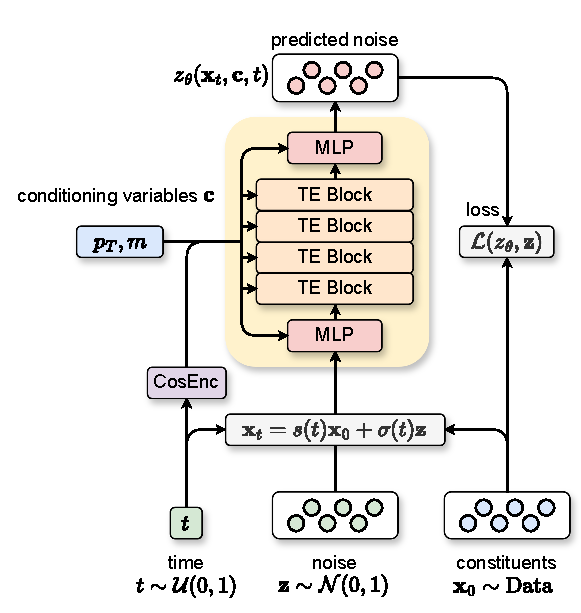
\includegraphics[width=0.65\textwidth]{Figures/jet_generation/pcjedi.pdf}
    \caption{The \pcjedi model architecture configured for training.}
    \label{fig:pcjedi}
\end{figure}

\subsubsection{Integration Solvers}

As with all diffusion models, to generate samples with \pcjedi, numerical integration is required to solve the reverse SDE or the probability flow ODE.
This complicates evaluation of the model, as sample quality can vary wildly depending on the solver used, and the number of integration steps taken.
We compared various numerical solvers for this task~\cite{NumericalSolutionStochastic}.
The Euler-Maruyama (EM) method was used to solve the reverse SDE, DDIM sampler~\cite{DDIM} was used for the probability-flow ODE.
We also experimented with the standard Euler solver and fourth-order Runge-Kutta methods but found negligible differences compared to DDIM.
Generating higher-quality jets requires more integration steps, which increases generation time as each step requires at least one forward pass through the model.
We focused on quality rather than speed, allowing 200 integration steps for each jet.
Equal step sizes were used for all solvers.

\subsection{Results}

As a benchmark for performance, we used MPGAN~\cite{MPGAN}, a GAN trained on the same dataset.
MPGAN generates the particle cloud with attributes $(\Delta\eta, \Delta\phi, \pt^\text{rel})$, where $\pt^\text{rel} = \pt / \ptjet$.
Thus, we transformed the outputs of \pcjedi to this format for comparison.
For evaluation, we generated 50k jets per class using MPGAN and \pcjedi using the different solvers.

Qualitative performance was assessed by visual inspection of the distributions of the generated jets compared to the JetNet30 test set.
For the distributions, we used the relative particle cloud kinematics, $\mpcrel$ and $\ptpcrel$, which were calculated using $\pt^\text{rel}$ for each constituent.
These distributions are shown in \Cref{fig:kinematics_gluon, fig:kinematics_top} gluon and top jets.
Total $\ptpcrel$ is not always 1.0 due to the top 30 constituents' selection, though this is the maximum physical value.
All generative models struggle to capture the hard cut-off at 1.0 in but \pcjedi with DDIM solver shows the closest agreement.
Both \pcjedi models outperform MPGAN in reconstructing the top jet $\pt$ distribution, with similar performance in reproducing $\mpcrel$ for both jet types.
The bi-modal structure observed in top jet $\mpcrel$ arises from a phenomenon in boosted top jet reconstruction where the stable particles from the $b$-quark decay are not contained within the radius of the jet.
These top jets are referred to as \emph{uncontained} top jets, and they exhibit a 2-pronged structure and masses close to the mass of the $W$~boson.

\begin{figure}[hbpt]
    \centering
    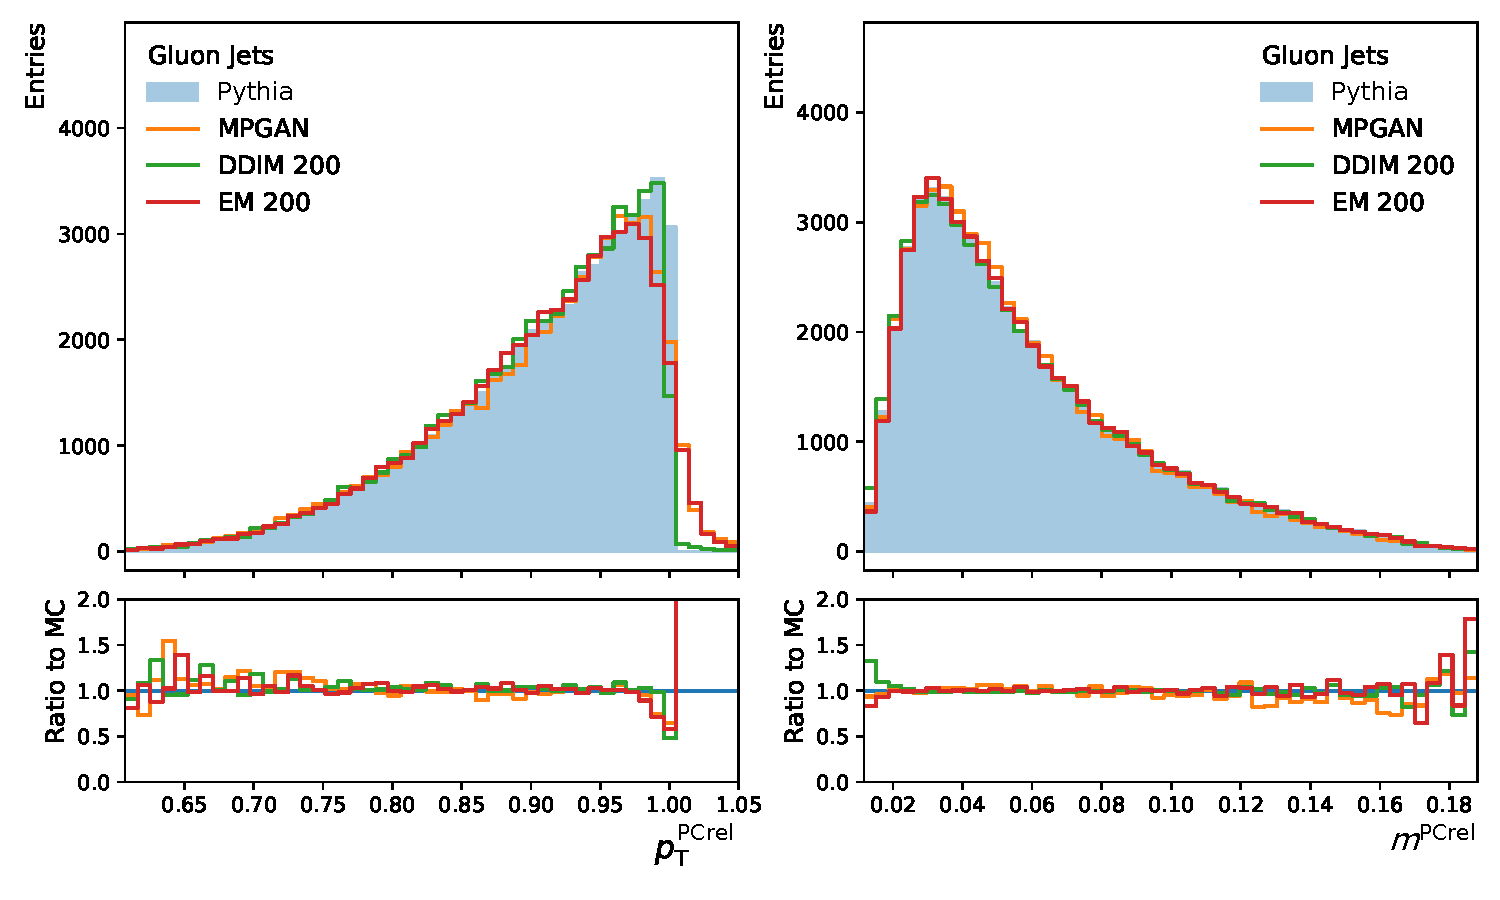
\includegraphics[width=.75\linewidth]{Figures/jet_generation/jedi/gluon/jet_features_rel.pdf}
    \caption{The relative transverse momentum (left) and invariant mass (right) of gluon jets generated with MPGAN and \pcjedi using the DDIM and EM solvers compared to the Pythia simulation. Calculated from the leading 30 \pt constituents using $\pt^\text{rel}$ instead of $\pt$.}
    \label{fig:kinematics_gluon}
\end{figure}

\begin{figure}[hbpt]
    \centering
    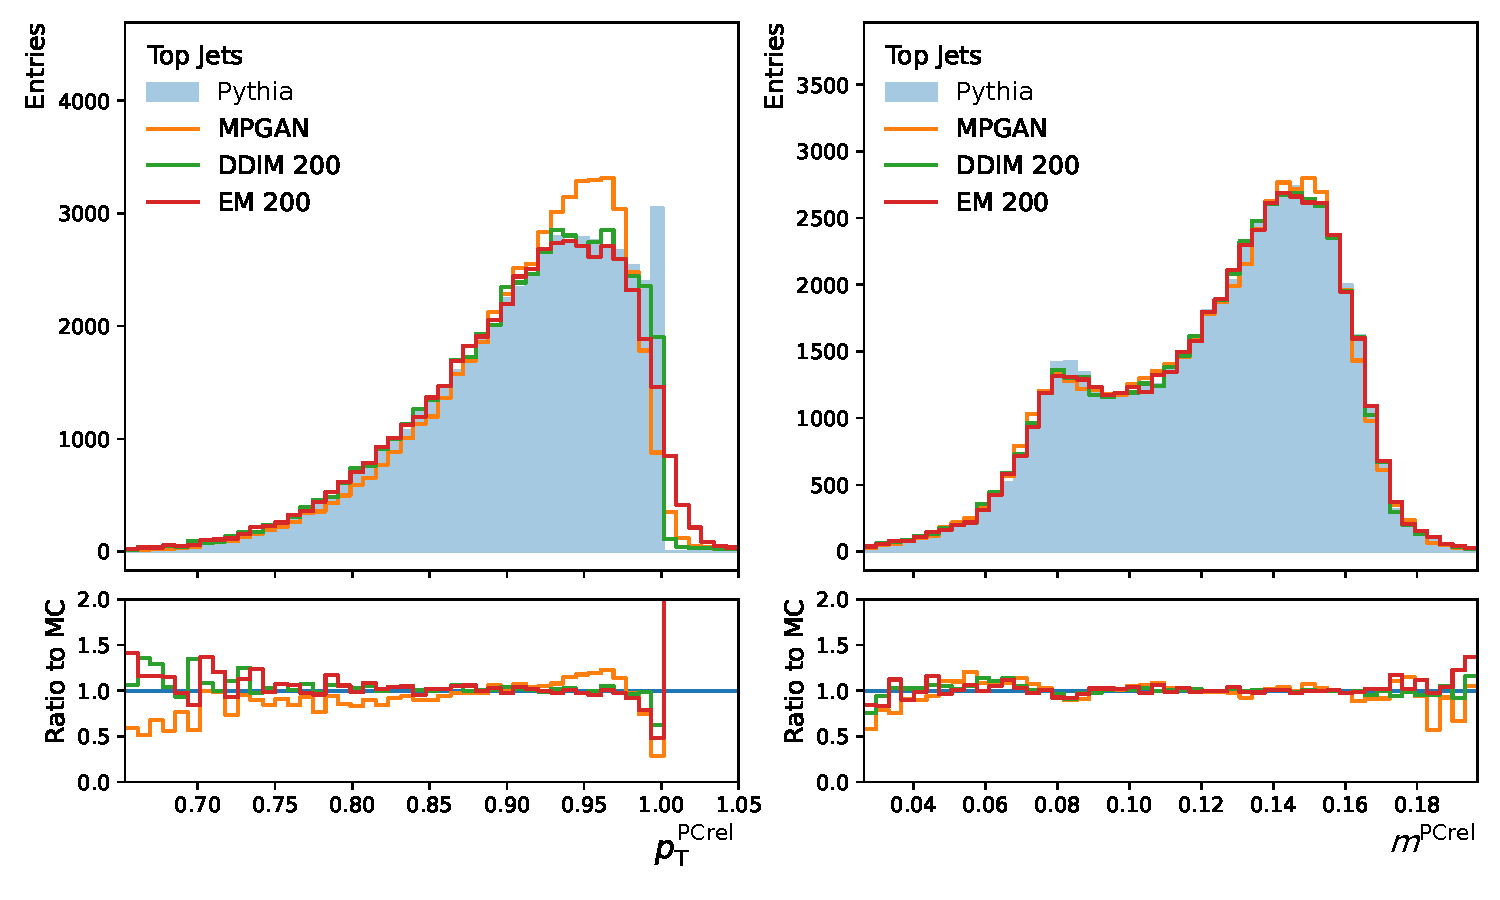
\includegraphics[width=.75\linewidth]{Figures/jet_generation/jedi/top/jet_features_rel.pdf}
    \caption{The relative transverse momentum (left) and invariant mass (right) of top jets generated with MPGAN and \pcjedi using the DDIM and EM solvers compared to the Pythia simulation. Calculated from the leading 30 \pt constituents using $\pt^\text{rel}$ instead of $\pt$.}
    \label{fig:kinematics_top}
\end{figure}

Crucial to the study of large-radius jets are the substructure variables $\tau_{21}$, $\tau_{32}$, and $D_2$ as described in \Cref{sec:jet_substructure}\footnote{These variables are already normalized by the jet's total $\pt$, thus relative versions are unnecessary.}.
The subjettiness ratios $\tau_{21}$, $\tau_{32}$ in particular are essential for distinguishing top jets from gluon or quark jets.
Calculated for the generated particle cloud and compared to Pythia simulations, these variables are illustrated in \Cref{fig:substructure_gluon, fig:substructure_top}.
Both \pcjedi and MPGAN models accurately captured the $\text{D}_2$ distributions.
However, all models struggled with $\tau_{21}$ and $\tau_{32}$ especially for top jets, which exhibits a bi-modal structure due to the uncontained $b$-quark decay.

\begin{figure}[hbpt]
    \centering
    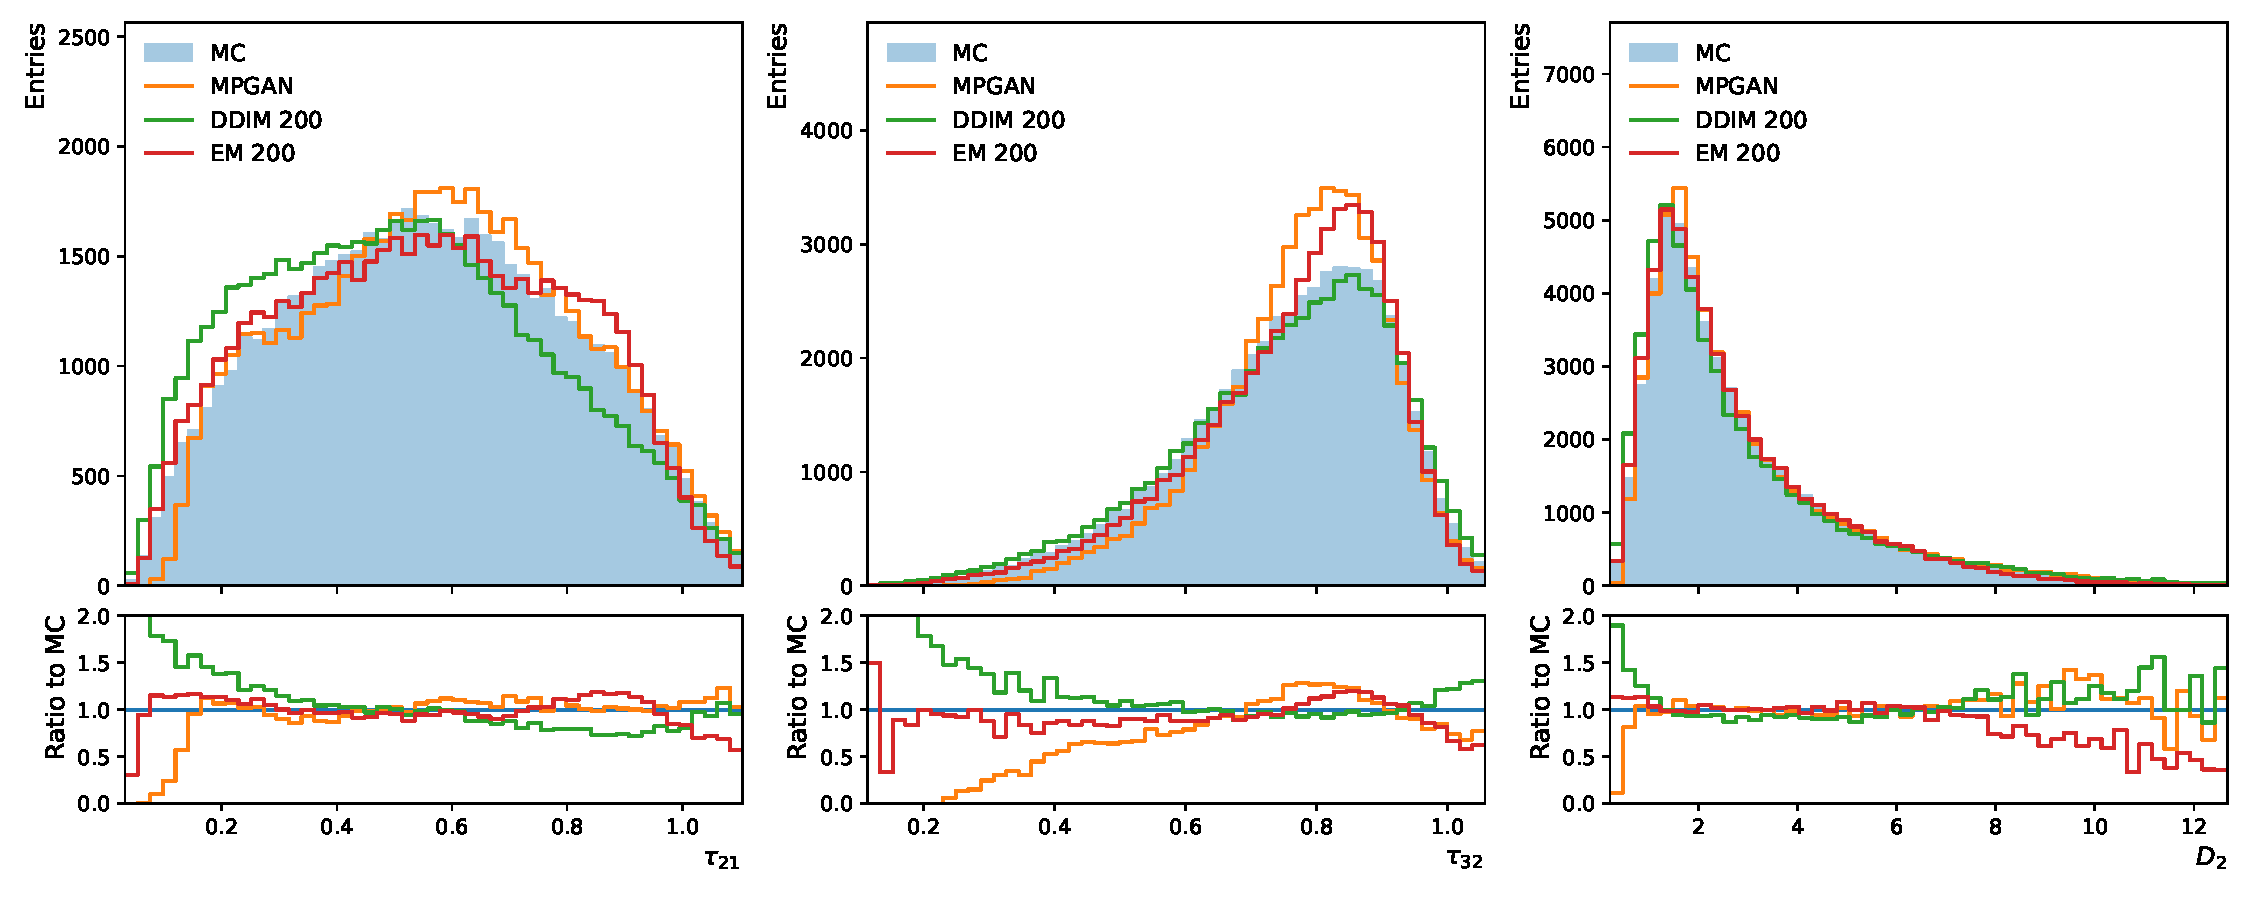
\includegraphics[width=1.\linewidth]{Figures/jet_generation/jedi/gluon/jet_substructure_rel.pdf}
    \caption{Substructure variables of gluon jets generated with MPGAN and \pcjedi using the DDIM and EM solvers compared to the Pythia.}
    \label{fig:substructure_gluon}
\end{figure}

\begin{figure}[hbpt]
    \centering
    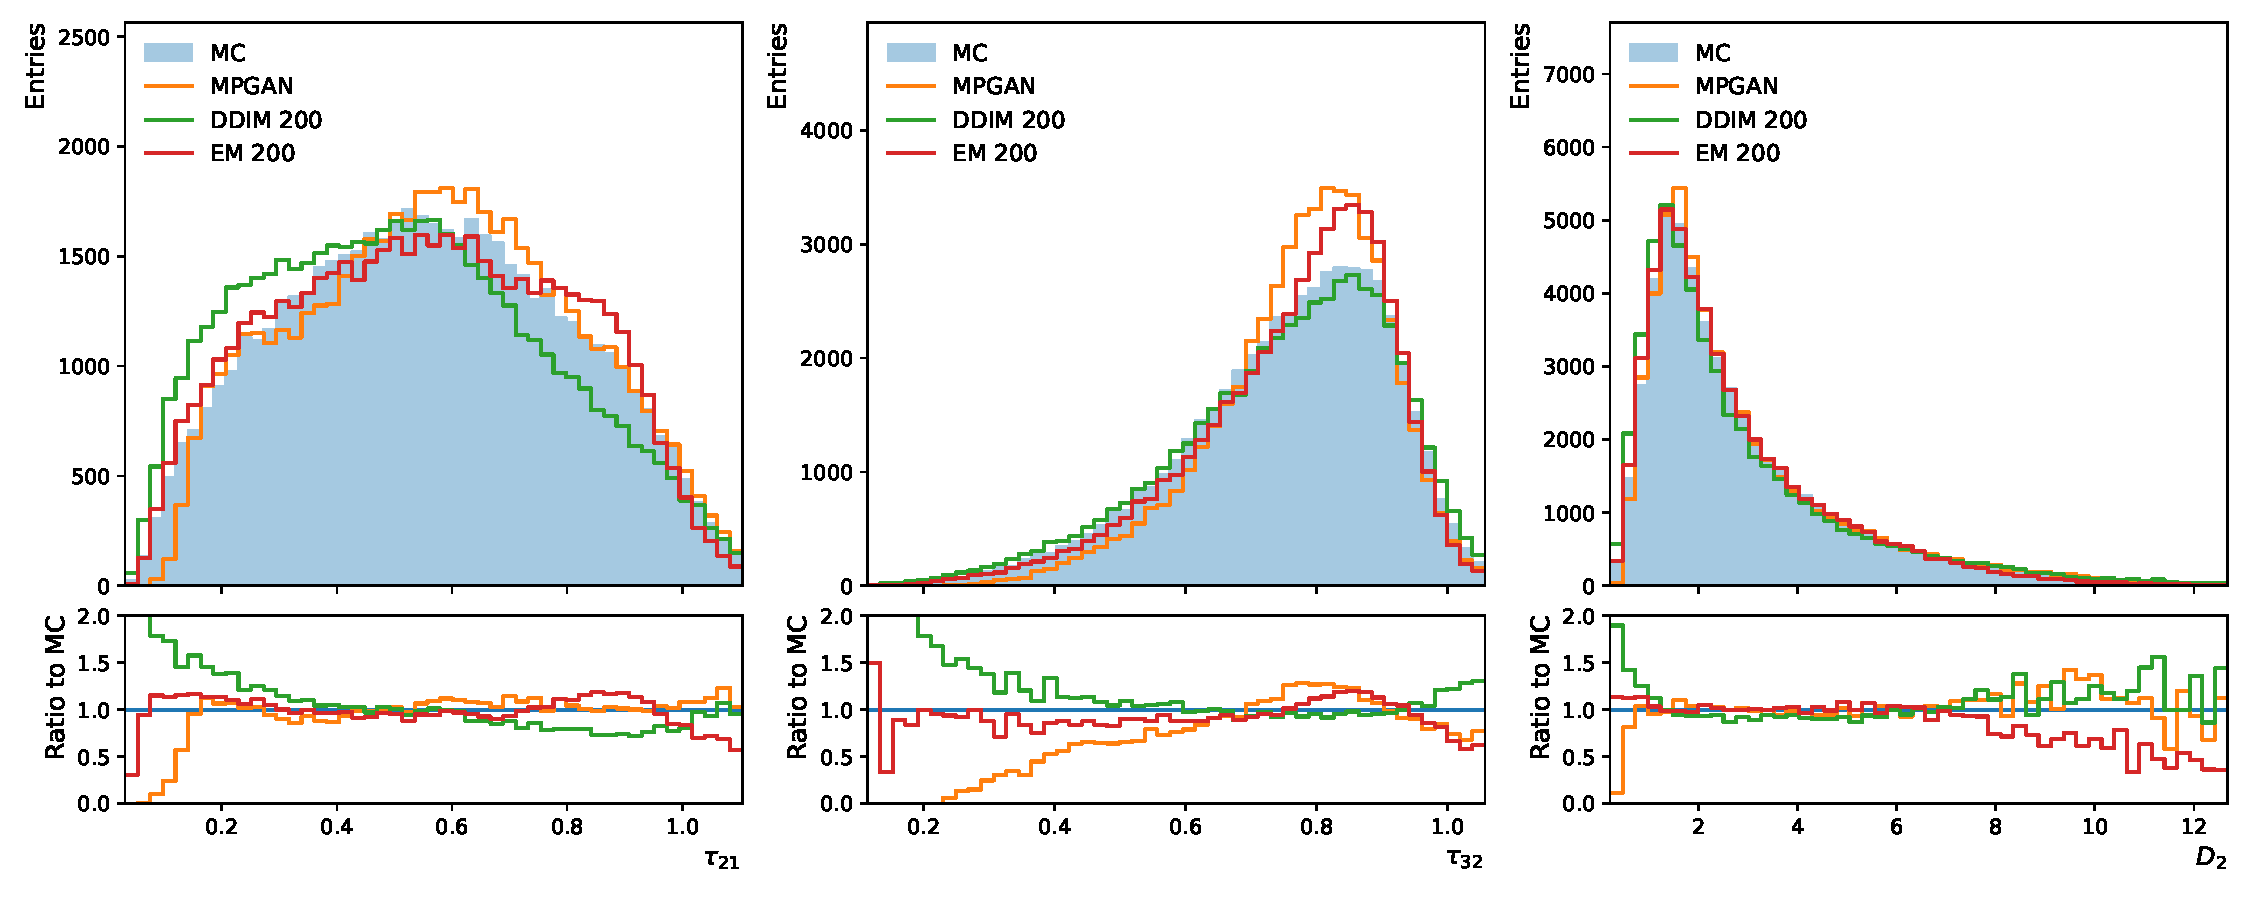
\includegraphics[width=1.\linewidth]{Figures/jet_generation/jedi/gluon/jet_substructure_rel.pdf}
    \caption{Substructure variables of top jets generated with MPGAN and \pcjedi using the DDIM and EM solvers compared to the Pythia simulation.}
    \label{fig:substructure_top}
\end{figure}

Quantitative metrics were derived following the methodology used in \textcite{MPGAN} whereby the Wasserstein-1 distance was calculated between the generated and Pythia jets, creating a $\text{W}_1$ score for each observable.
Uncertainties for these scores were derived using bootstrap sampling.
In addition to the distributions shown, we also calculated the $\text{W}_1$ score using the average of the first five Energy Flow Polynomials (EFPs)~\cite{EFP}, as these variables too are sensitive to the jet substructure.
Additionally, we computed the Fréchet ParticleNet distance (FPND), which compares the mean and standard deviation of the penultimate layer of the ParticleNet model for the Pythia and generated jets~\cite{MPGAN, ParticleNet}.
Lower limits for these values were calculated by comparing 50k jets from the training set to the test set, which captures the natrual variation in the data.
This allows us to compare the various methods quantitatively in \Cref{tab:kansal_results}.
Based on these value, no one model is clearly superior.
\pcjedi with the EM sampler obtains the superior FPND score, but suffers greatly in the EFP distributions for top jets.
MPGAN outperforms \pcjedi in the $\Dtwo$ scores for gluon jets but not for top jets.
On average, it seems that the EM sampler is worse than the DDIM sampler, at least for the selected 200 integration steps, but the differences are not significant.
One crucial observation is how poorly all models perform on the subjetiness ratios with the ratio to Pythia for top jets, ranging from around 5 to 10 times higher than the MC-MC comparison.
This clearly indicates that the current methods are not sufficient for modelling the substructure of the large radius jets.

\begin{table}[hbpt]
    \centering
    \caption{Quantative comparison of the \pcjedi and MPGAN models for generating gluon and top jets.}
    \label{tab:combined_results}
    \renewcommand{\arraystretch}{1.5}
    \resizebox{\textwidth}{!}{
        \begin{tabular}{llrrrrrr}
    \toprule
    Jet & Model        & FPND            & $\mathrm{W}_1^\mathrm{EFP}$ $(\times 10^{-6})$ & $\mathrm{W}_1^m$ $(\times 10^{-4})$ & $\mathrm{W}_1^{\tau_{21}}$ $(\times 10^{-3})$ & $\mathrm{W}_1^{\tau_{32}}$ $(\times 10^{-3})$ & $\mathrm{W}_1^{\Dtwo}$ $(\times 10^{-2})$ \\
    \midrule
    \multirow{4}{*}{Top}
        & \pythia      & $0.01$          & $8.07 \pm 3.51$                                & $3.23 \pm 1.07$                     & $2.01 \pm 0.74$                               & $2.90 \pm 1.59$                               & $1.16 \pm 0.29$                           \\ \cline{2-8}
        & \pcjedi-EM   & $\mathbf{0.15}$ & $35.61 \pm 4.92$                               & $13.64 \pm 3.21$                    & $4.55 \pm 1.16$                               & $\mathbf{16.05} \pm 1.31$                     & $\mathbf{2.08} \pm 0.40$                  \\
        & \pcjedi-DDIM & $0.28$          & $41.21 \pm 5.61$                               & $14.82 \pm 3.21$                    & $\mathbf{4.40} \pm 1.03$                      & $32.04 \pm 2.29$                              & $2.59 \pm 0.41$                           \\
        & MPGAN        & $0.36$          & $\mathbf{12.80} \pm 4.89$                      & $\mathbf{6.41} \pm 2.09$            & $6.61 \pm 0.92$                               & $17.41 \pm 2.78$                              & $3.40 \pm 0.63$                           \\
    \midrule
    \multirow{4}{*}{Gluon}
        & \pythia      & $0.01$          & $4.07 \pm 1.27$                                & $4.39 \pm 1.59$                     & $3.79 \pm 1.42$                               & $2.26 \pm 0.51$                               & $3.78 \pm 0.70$                           \\ \cline{2-8}
        & \pcjedi-EM   & $\mathbf{0.10}$ & $5.68 \pm 1.09$                                & $\mathbf{5.66} \pm 1.51$            & $12.48 \pm 0.98$                              & $\mathbf{13.32} \pm 0.96$                     & $10.20 \pm 1.04$                          \\
        & \pcjedi-DDIM & $0.12$          & $\mathbf{5.10} \pm 0.99$                       & $9.04 \pm 1.77$                     & $\mathbf{11.99} \pm 1.12$                     & $20.38 \pm 1.91$                              & $11.39 \pm 1.42$                          \\
        & MPGAN        & $0.13$          & $8.76 \pm 2.44$                                & $8.15 \pm 2.10$                     & $16.83 \pm 2.08$                              & $25.27 \pm 1.29$                              & $\mathbf{5.64} \pm 1.01$                  \\
    \bottomrule
\end{tabular}

    }
\end{table}

\subsection{Discussion}

\pcjedi was the first model to generate particle clouds using a diffusion model, and while the results were promising, they were not state-of-the-art.
However, proving that the method could work was a significant step forward.
Furthermore, the time required to generate samples with diffusion models is another drawback, as it requires multiple forward passes compared to a single pass for a GAN.
The following steps in this research would be to improve the model's performance and speed.

\section{\pcdroid}

This section details the advancements made with \pcdroid, a successor to \pcjedi~\cite{PCDroid}.
The \pcdroid model exhibits marked improvements in speed and generation.
Leveraging an updated framework for diffusion models~\cite{ElucidatingDesignSpace}, enhanced diffusion sampling algorithms, and a novel transformer model, \pcdroid better balances performance and generation time.
Additionally, we explored using consistency distillation~\cite{ConsistencyModels} to even further reduce generation time.
\pcdroid achieves state-of-the-art performance on the benchmarks discussed in the previous section, notably surpassing both \pcjedi and MPGAN.
We also included much more elaborate timing studies to compare the various models against performing the showering using \pythia.
The code repository used in this work is publicly available~\cite{PCDroidCode}.

\subsection{Improved Diffusion Framework}

One of the main advancements in \pcdroid is the revised diffusion paradigm and configuration.
\pcdroid adheres to the EDM noise scheduler and network preconditioning as outlined by \textcite{ElucidatingDesignSpace}, discussed in \Cref{sec:diffusion_frameworks}.
This approach introduces several key modifications.

Firstly, the signal and noise rates are defined as $\gamma(t)=1$ and $\sigma(t)=t$.
This adjustment simplifies the forward SDE to
\begin{equation}
    \diff \x_t = \sqrt{2t} \diff \w_t,
\end{equation}
with the corresponding ordinary differential equation ODE similarly reducing to,
\begin{equation}
    \diff x_t = - t \score \diff t.
\end{equation}
As a result, the ODE solutions exhibit straighter trajectories, reducing truncation errors during generation compared to the previous variance-preserving method.
The primary advantage of this change is the ability to execute the reverse diffusion process in fewer steps.

Secondly, diffusion times are sampled during training specifically to target regions of the diffusion process where the model can gain the most information.
These diffusion times are used to scale the noise added to the input data.
Note that the diffusion time $t$ and noise rate $\sigma(t)$ can be used interchangeably, with $t$ extending beyond the range of 0 to 1, instead falling in the range $t = \sigma(t) \in [0, 80]$.
When $t$ is low, the magnitude of the artificial noise introduced into the samples is indistinguishable from the inherent stochasticity of the data.
Conversely, at high values of $t$, the input sample is almost entirely corrupted by noise, and the model can at most return the mean of the data distribution.
Log-normal sampling of the diffusion times, ${\log(t)\sim\mathcal{N}\left(-1.2, 1.2\right)}$, preferentially targets intermediate values where the model can learn the most.
This specific sampling distribution~\cite{ElucidatingDesignSpace} was observed to be advantageous for our tasks.

Thirdly, sophisticated skip and scaling connections are integrated into the network architecture.
The variables $c_\mathrm{in}(t)$, $c_\mathrm{out}(t)$, and $c_\mathrm{skip}(t)$ are all parameterized by $t$ and are combined for the denoised estimate as follows:
\begin{equation}
    x_\theta(\x, \cond, t) = c_\mathrm{out} f_\theta(c_\mathrm{in}\x, \cond, t) + c_\mathrm{skip}\x,
\end{equation}
where $f_\theta$ represents the raw prediction from the neural network.
Note that unlike \pcjedi, the target for the network is the true data sample $\x_0$ rather than the noise $\z$.
The skip connection permits $\x_t$ to bypass the network at low $t$, as the input is inherently closer to the target.
Due to the variance not being preserved during the diffusion process, these  scaling functions maintain the unit variance of the raw inputs and targets
for $f_\theta$.

We reuse the same dataset, JetNet30, as outlined in \Cref{sec:jetgen_data} for some experiments in this section.
However, most of the studies are performed using the extended JetNet150 dataset, which encompasses the same jets but with up to 150 constituents within the particle cloud.
This expanded dataset poses new challenges for the generative task, necessitating more intricate models and increased computational resources to manage the larger set size effectively.
Furthermore, we used all five jet types in JetNet150, rather than just the gluon and top jets.

\subsection{Model Architecture}

The general \pcdroid architecture and the training process is shown in \cref{fig:droid_arch_train}.

In addition to the preconditioning which comes from the EDM framework, the model has an additional MLP compared to \pcjedi which processes the conditional input before sending it to each sublayer.
This is primarily because the number of context variables increased to also include the jet azimuthal angle ($\phi$), the number of constituents (which was previously only implicitly included in the input set size), and the jet type (PID).
This last feature is significant because, whereas \pcjedi and MPGAN required separate models for each jet type, \pcdroid can generate all five jet types with a single conditional network.
Furthermore, the conditioning features represent the full jet kinematics, rather than just the net kinematics of the particle cloud.
This makes the generation a more challenging task, as it would have to learn the effects of truncating the particle cloud.

\begin{figure}[htpb]
    \centering
    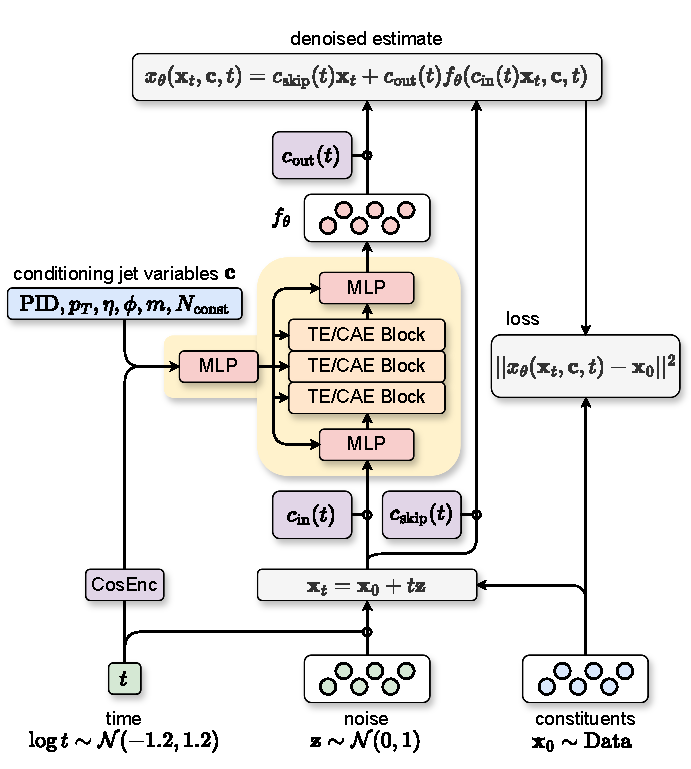
\includegraphics[width=0.6\textwidth]{Figures/jet_generation/pcdroid.pdf}
    \caption{The \pcdroid model architecture configured for training.}
    \label{fig:droid_arch_train}
\end{figure}

In \pcjedi, only TE Blocks with self-attention were studied, which, despite their high expressiveness, are computationally expensive.
The number of operations scales quadratically with the number of constituents $N_{const}$, i.e., $\mathcal{O}(N_{const}^2)$.
Given that diffusion models necessitate multiple network passes during generation, self-attention becomes a suboptimal choice for fast generation.
While this computational demand is manageable for models with 30 constituents, it becomes significantly impactful when scaling to 150 constituents.
Consequently, alongside the TE based model, we introduce the cross-attention encoder (CAE), which serves as a more efficient and memory-conserving permutation-equivariant network.

A schematic overview of the CAE Block is illustrated in \Cref{fig:cae_network}.
In a CAE Block, the input particle cloud updates a set of global tokens via multi-headed cross-attention, with the number of global tokens $N_{global}$ serving as a hyperparameter.
These tokens are then refined through a residual MLP and redistributed back to the point cloud using another cross-attention layer and residual MLP.
The full CAE is constructed by sequentially stacking multiple CAE Blocks, with the initial set of global tokens being fully learnable.
For $N_{global}=1$, the distribution attention operation employs a sigmoid function instead of softmax.
The CAE's attention operations scale with $\mathcal{O}(N_{const} \times N_{global})$.
The first attention operation effectively pools information from the point cloud into the global tokens. The second attention operation is inverted, and information from the updated global token are distributed back to the point cloud.

\begin{figure}[htpb]
    \centering
    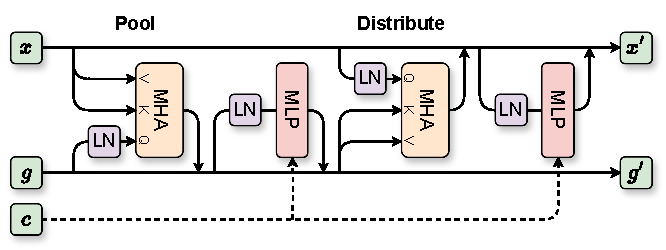
\includegraphics[width=0.8\textwidth]{Figures/jet_generation/CAEB.pdf}
    \caption{A single cross-attention encoder block updating both an input point cloud $x$ and global tokens $g$, using layer-norm (LN), multi-headed attention (MHA). Contextual information $c$ is injected into the network by concatenating to the inputs of the MLPs.}
    \label{fig:cae_network}
\end{figure}

To allow direct comparisons with \pcjedi, the optimizer, learning rate, scheduler, and the majority of hyperparameters remain unchanged.
The only notable adjustments, based on a minor hyperparameter scan, include reducing the number of encoder layers from four to three and using MSE loss for training.
For models with 150 constituents, the token dimension and the width of the MLP layers were doubled.
We trained two additional models utilizing CAE Blocks with $N_{global}=1$ and 16, on the 150 constituent dataset, employing the same training configuration, dimensions, and number of layers as the baseline model.

\subsubsection{Integration Solvers}

Another key development has been in the choice of integration solvers used during inference.
Several state-of-the-art algorithms have been studied and \pcdroid was designed to be compatible with the popular \textsc{K-Diffusion} library~\cite{KDiffusion}.
The most promising solvers include a fourth order linear multistep method (LMS)~\cite{ODEBook}, DPM-Solver-2~\cite{DPMSolverFastODE}, DPM-Solver++~\cite{DPMSolverFastSolver}, and DPM-Solver-2M~\cite{DPMSolverFastSolver}, and ancestral variants of these.
Furthermore, we experimented with non-uniform step sizes during generation, and found that systematically taking larger steps at the beginning of the denoising process and smaller steps towards the end improved the quality of the generated samples.

\subsection{Consistency Distillation}

Additionally, this work investigated the process of consistency distillation (CD) \cite{ConsistencyModels}, wherein a teacher network trains a student network to solve the reverse diffusion process in fewer steps, and in some cases enabling \textit{one-shot} generation.

The teacher network is a standard pre-trained diffusion model which together with a sampling method, defines a method to trace paths along the learned probability flow ODE.
During distillation, the weights of the teacher network are frozen, and a student network is trained to map all points sampled along a same ODE trajectory a common target.
To prevent the student model from collapsing into a constant function, a boundary condition is enforced such that the student must become an identity map as the diffusion time approaches zero.
The same skip connections used in the \pcdroid model are employed to enforce this.
This boundary condition ensures the global minimum of the training loss was achieved only when the student network mapped each point of the ODE trajectory to its endpoint.

Initially, the student model is initialized with the same parameter values as the teacher model.
During training, the diffusion time is sampled, the input is corrupted using the same schedule as before, and then the teacher model is used to take a single step along the ODE.
These two adjacent points on the ODE are each passed through the student network, and the student is trained to minimize the mean squared distance between its two outputs.
To stabilize training, the student network was duplicated into an online and target network, a practice common in deep reinforcement learning \cite{PlayingAtariDeep, ContinuousControlDeep, ImplicitQuantileNetworks}.
Gradients propagated only through the online network, which always processed the ODE sample with the larger $t$.
After each iteration, the target network was synced with the student network using an EMA of the parameters.

Although both are distillation methods, CD differs from progressive distillation models (PD) \cite{ProgressiveDistillationFast}.
In progressive distillation, new models are iteratively trained to predict the amount of noise removed in $N$ steps of the previous model.
This iterative process reduces the overall number of steps required with each new model, thereby resulting in faster generation times.
Unlike CD, PD does not require information about the ODE trajectories, only the total amount of noise removed after $N$ steps.

\subsection{Unconditional Generation}

\pcdroid is trained as a conditional generative model, with the jet kinematics $(\pt, \eta, m)$, the number of constituents ($N_{const}$), and the PID used as conditions.
We can marginalize the conditional variables using a second generative model to allow for unconditional generation.
As this is a low-dimensional vector, we trained NFs for this task.
This approach is preferable to explicitly unconditional models as it logically segments the learning process.

Standard use cases would still demand control over the jet type, so
one flow (Flow-$\p$) is trained to learn the probability density $p(\pt, \eta, m, N_{const} |\textrm{PID})$.
A second flow (Flow-$N$) is trained to learn the probability density $ p(N_{const}|\pt, \eta, m, \textrm{PID}) $.
This second flow demonstrates how \pcdroid can be used as a surrogate fast simulator, especially when the parton type and kinematics are known, but the number of particles in the final jet is not.
As the transformer denoises all input tokens, the number of constituents is always required at generation time.
This number is correlated to many jet properties, necessitating a normalizing flow rather than simply sampling from a Poisson distribution.

Both flows are trained with a maximum log-likelihood objective and consist of five transformation layers using rational quadratic splines~\cite{NeuralSplineFlows}.
Coupling layers are used in Flow-$\p$, while none are needed for the one-dimensional transformation Flow-$N$.
For both flows, a dequantization step simplifies the learning of the $N_{const}$ distribution; at inference time, the generated value is rounded to the nearest integer.
The Adam optimizer~\cite{Adam} with default settings and a cosine learning rate is used.
Given the relatively simple nature of these distributions, near-perfect performance is achieved using only four layers and 100k learnable parameters.

\subsection{Results}

\subsubsection{JetNet30}

We compared the \pcdroid, \pcjedi, and MPGAN models on the JetNet30 dataset using the same distributions and metrics as before.
This study utilized \pcdroid samples generated under the fully conditional regime.
Performance comparison revealed minimal differences between jets conditioned on the training set kinematics and those conditioned on the flow outputs.

We test a wide variety of integration solvers in the generation stage for \pcjedi.
We studied the trade-off between the quality of generated jets and the number of neural function evaluations (NFE) to determine the optimal solver and step size.
The comparison focused on the FPND, $\mathrm{W}_1^M$, and $\mathrm{W}1^{\tau{32}}$ metrics, given the latter's difficulty in previous studies.
For \pcjedi we used the results using the Euler-Maruyama sampler at 200 NFE.
From \cref{fig:metrics_vs_steps-30}, we observe most solvers saturating around 100 NFE.
We generated samples with \pcdroid using Heun and HeunSDE methods~\cite{ElucidatingDesignSpace}, DPM2~\cite{DPMSolverFastODE}, DPM2 with ancestral sampling (DPM2A), DPM++2M~\cite{DPMSolverFastSolver}, and LMS~\cite{ODEBook}
Although no method was clearly superior, the LMS solver generally performed best across most metrics, and was thus used at 100 NFE for all \pcdroid results in the following sections.
Additionally, \pcdroid outperformed MPGAN with as few as 20 steps for most solvers.

\begin{figure}[htpb]
    \centering
    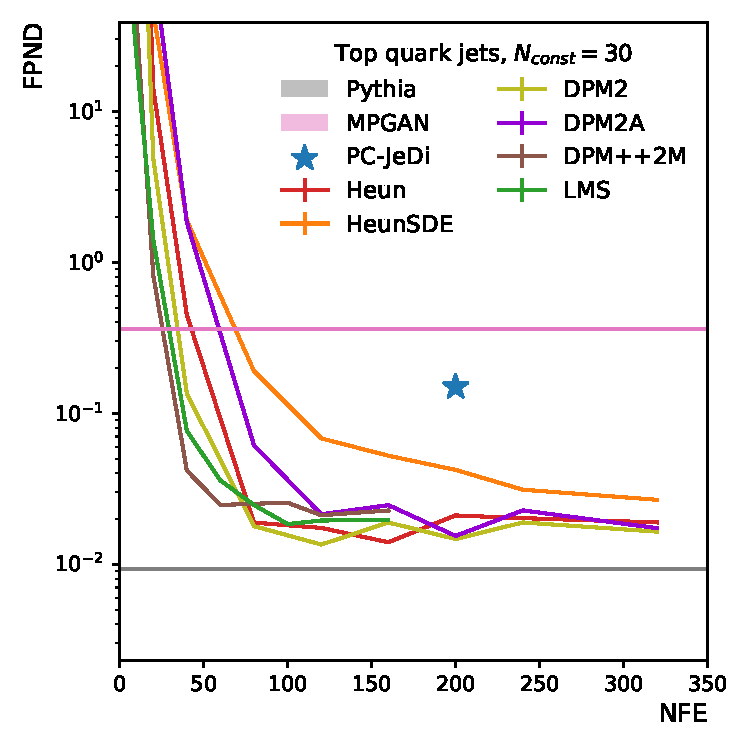
\includegraphics[width=0.32\linewidth]{Figures/jet_generation/droid/30/metrics_vs_steps/t/t_fpnd.pdf}
    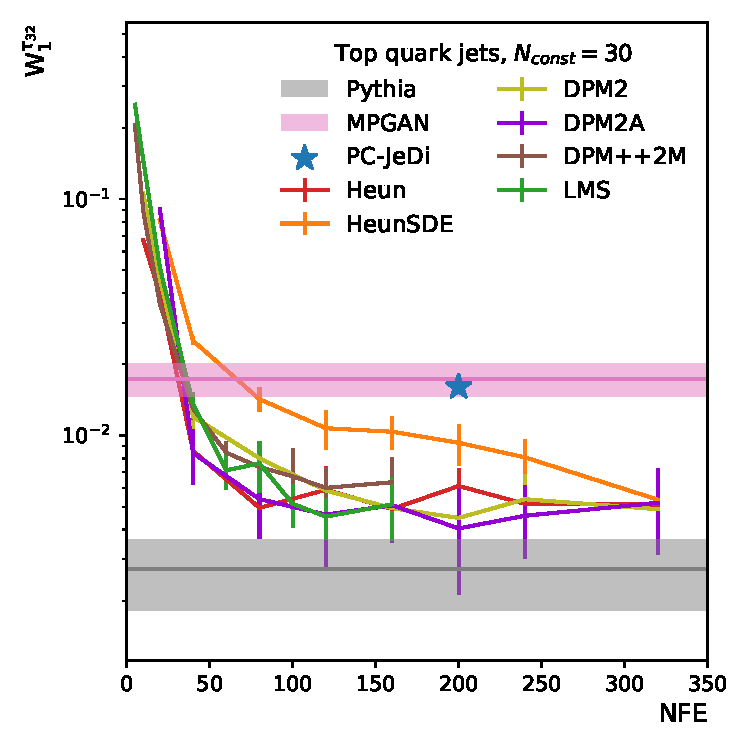
\includegraphics[width=0.32\linewidth]{Figures/jet_generation/droid/30/metrics_vs_steps/t/t_w1_tau_32.pdf}
    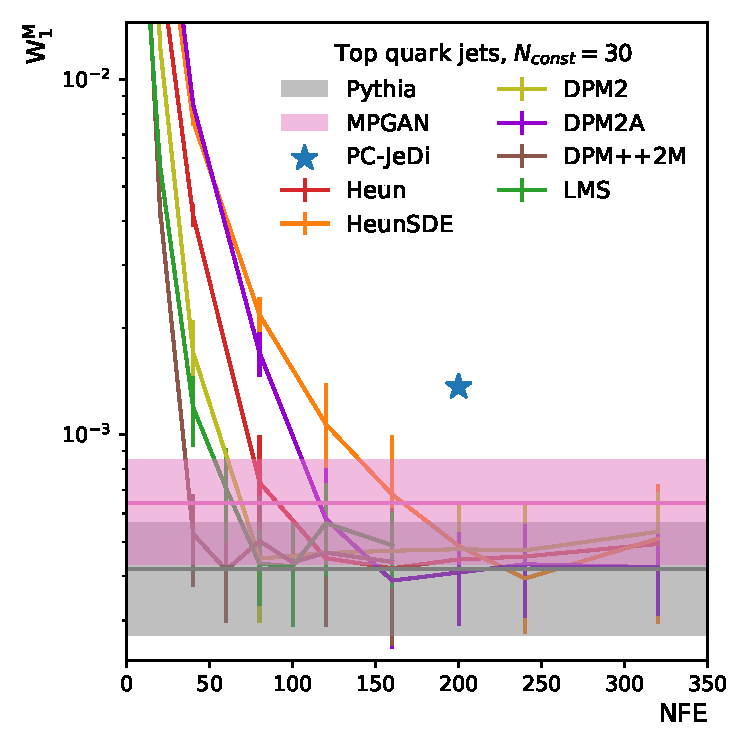
\includegraphics[width=0.32\linewidth]{Figures/jet_generation/droid/30/metrics_vs_steps/t/t_w1m.pdf}
    \caption{Performance as measured by FPND (left), W$_1^{\tau_{32}}$ (middle), and W$_1^\mathrm{M}$ (right) as a function of the NFE used during generation for the \pcdroid model for top jets with up to 30 constituents.}
    \label{fig:metrics_vs_steps-30}
\end{figure}

Effectively modelling the kinematics of individual constituents is essential for jet generation.
\Cref{fig:const-pt_dist-30} illustrates the \pt distributions of the leading, fifth leading, and twentieth leading constituents of the generated top and gluon jets, as represented by \pcdroid and \pcjedi.
\pcdroid shows better alignment with Pythia compared to \pcjedi across all constituents, especially in the distribution tails.

\begin{figure*}[htpb]
    \centering
    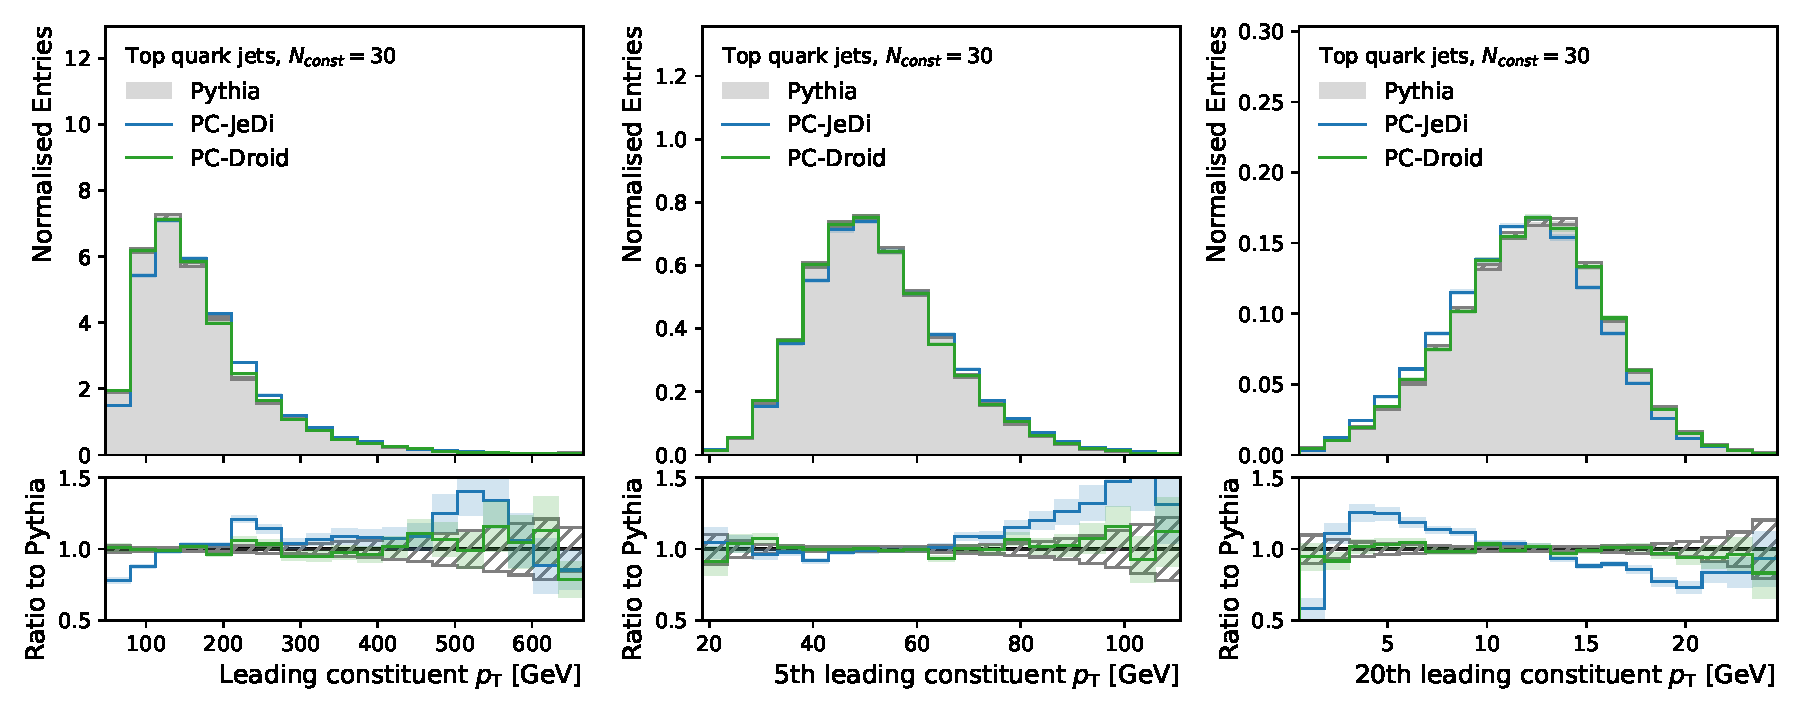
\includegraphics[width=0.99\linewidth]{Figures/jet_generation/droid/30/csts/t/100/t_leading_constituents.pdf} \\
    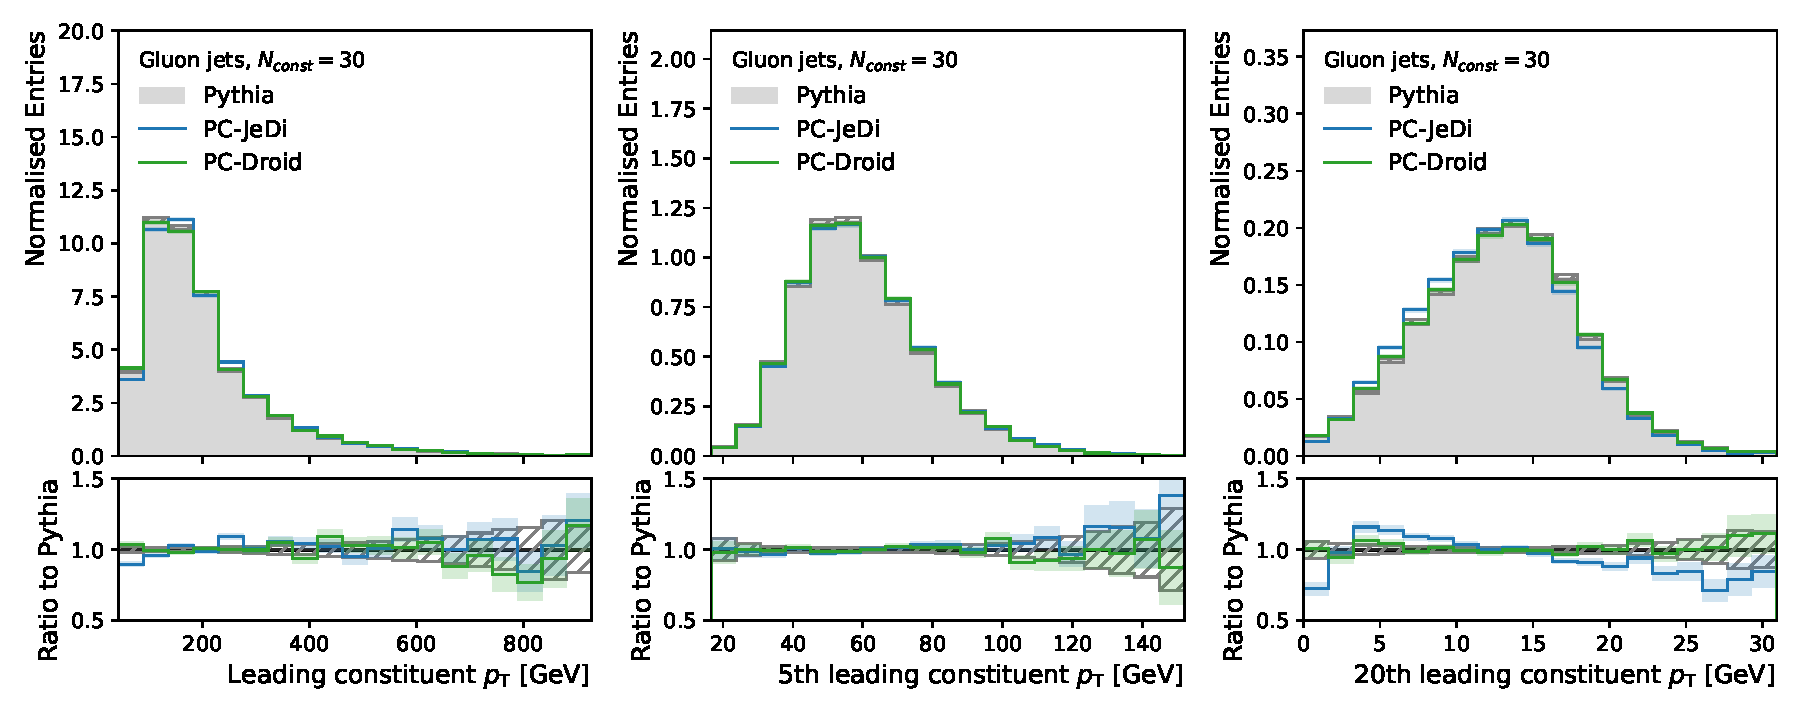
\includegraphics[width=0.99\linewidth]{Figures/jet_generation/droid/30/csts/g/100/g_leading_constituents.pdf}
    \caption{Comparison of \pt distributions of the leading, fifth leading, and twentieth leading constituents of the generated top and gluon jets with up to 30 constituents.}
    \label{fig:const-pt_dist-30}
\end{figure*}

Next, we examine the substructure variable distributions of the generated jets and their correlations, essential for jet tagging.
We focus on top jets due to their complex substructure, which has proven challenging to model.
\Cref{fig:hlvs-30} shows that \pcdroid significantly improves $\tau_{32}$ modelling compared to \pcjedi and aligns excellently with Pythia simulations for all other substructure variables.
\begin{figure*}[htpb]
    \centering
    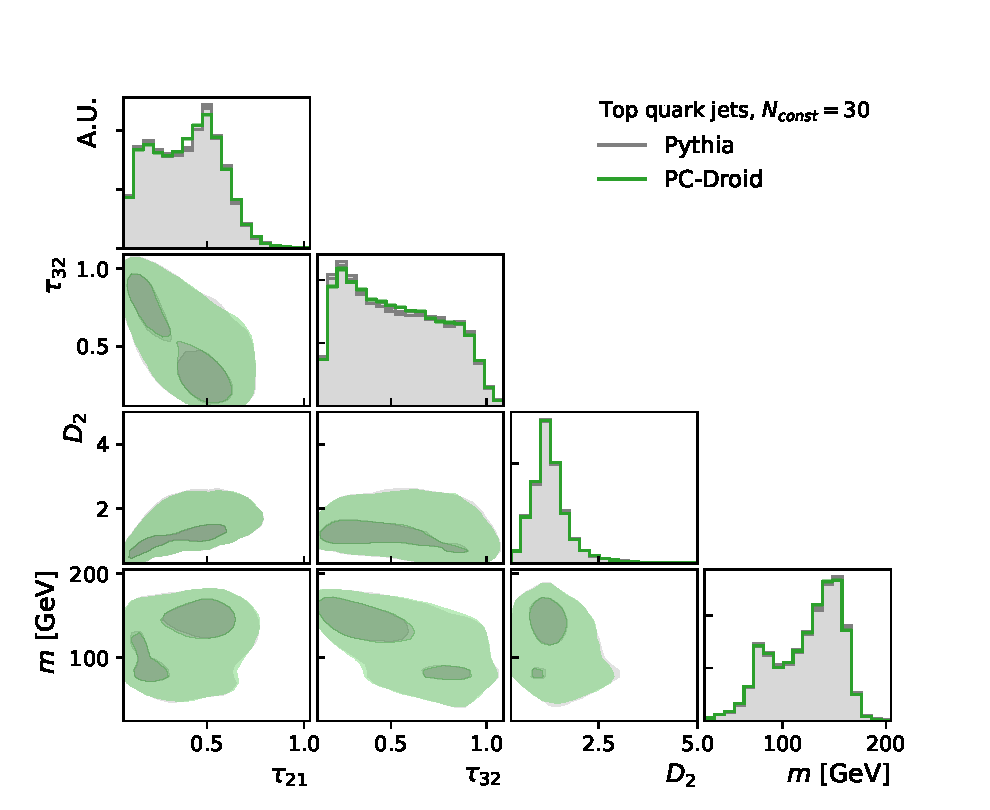
\includegraphics[width=0.49\linewidth]{Figures/jet_generation/droid/30/hlvs/t/100/hlv_corr_PC-Droid.pdf}
    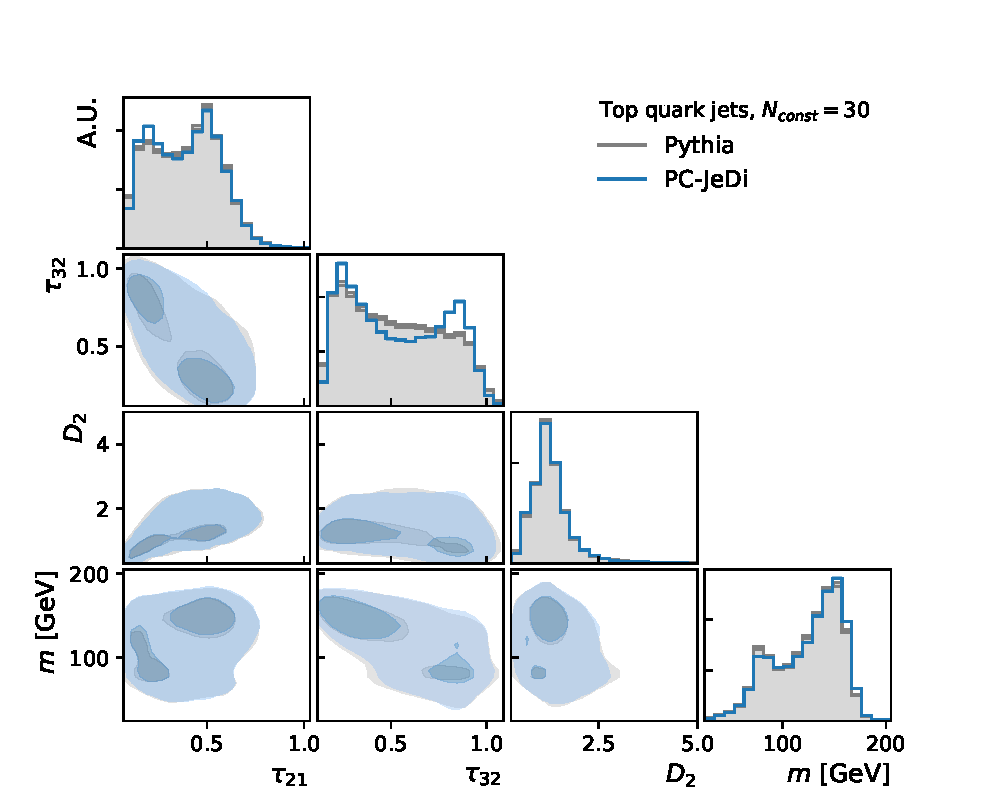
\includegraphics[width=0.49\linewidth]{Figures/jet_generation/droid/30/hlvs/t/100/hlv_corr_PC-Jedi.pdf}
    \caption{
        Mass and substructure distributions of the generated top jets with up to 30 constituents.
        The diagonal consists of the marginals of the distributions and the off-diagonal elements contain the joint distributions.
    }
    \label{fig:hlvs-30}
\end{figure*}

The generation performance is summarized in~\cref{tab:30_table} for gluon and top jets.
The $\mathrm{W_1^P}$ score describes the average Wasserstein-1 distance between the marginal distributions of the generated and Pythia constituent kinematics.
Particularly in FPND, \pcdroid surpasses all other methods in all metrics, reaching the intra MC-MC comparison limits in the subjettiness ratios for gluons and $\mathrm{W_1^{D_2}}$ for both jet types.

\begin{table*}[tp]
    \centering
    \caption{Comparison of generative models on top and gluons with up to 30 constituents. Lower is better.}
    \label{tab:30_table}
    \resizebox{\textwidth}{!}{%
        \begin{tabular}{llrrrrrrr}
    \toprule
    Jet & Model    & FPND            & $\mathrm{W_1^P}$ $(\times 10^{-4})$ & $\mathrm{W}_1^\mathrm{EFP}$ $(\times 10^{-6})$ & $\mathrm{W}_1^m$ $(\times 10^{-4})$ & $\mathrm{W}_1^{\tau_{21}}$ $(\times 10^{-3})$ & $\mathrm{W}_1^{\tau_{32}}$ $(\times 10^{-3})$ & $\mathrm{W}_1^{\Dtwo}$ $(\times 10^{-2})$ \\
    \midrule
    \multirow{4}{*}{Top}
        & \pythia  & $0.01$          & $3.98 \pm 1.27$                     & $8.07 \pm 3.51$                                & $3.23 \pm 1.07$                     & $2.01 \pm 0.74$                               & $2.90 \pm 1.59$                               & $1.16 \pm 0.29$                           \\ \cline{2-9}
        & \pcdroid & $\mathbf{0.02}$ & $\mathbf{5.02 \pm 1.59}$            & $\mathbf{11.59 \pm 3.29}$                      & $\mathbf{4.27 \pm 1.39}$            & $\mathbf{2.91 \pm 1.09}$                      & $\mathbf{5.14 \pm 1.06}$                      & $\mathbf{1.26 \pm 0.33}$                  \\
        & PC-JeDi  & $0.15$          & $12.07 \pm 2.01$                    & $35.61 \pm 4.92$                               & $13.64 \pm 3.21$                    & $4.55 \pm 1.16$                               & $16.05 \pm 1.31$                              & $2.08 \pm 0.40$                           \\
        & MPGAN    & $0.36$          & $21.73 \pm 2.02$                    & $12.80 \pm 4.89$                               & $6.41 \pm 2.09$                     & $6.61 \pm 0.92$                               & $17.41 \pm 2.78$                              & $3.40 \pm 0.63$                           \\
    \midrule
    \multirow{4}{*}{Gluon}
        & \pythia  & $0.01$          & $3.54 \pm 1.19$                     & $4.07 \pm 1.27$                                & $4.39 \pm 1.59$                     & $3.79 \pm 1.42$                               & $2.26 \pm 0.51$                               & $3.78 \pm 0.70$                           \\ \cline{2-9}
        & \pcdroid & $\mathbf{0.01}$ & $\mathbf{3.66 \pm 1.07}$            & $\mathbf{4.13 \pm 1.61}$                       & $\mathbf{4.48 \pm 1.47}$            & $\mathbf{2.89 \pm 0.80}$                      & $\mathbf{1.99 \pm 0.51}$                      & $\mathbf{3.52 \pm 1.33}$                  \\
        & PC-JeDi  & $0.10$          & $5.83 \pm 1.44$                     & $5.68 \pm 1.09$                                & $5.66 \pm 1.51$                     & $12.48 \pm 0.98$                              & $13.32 \pm 0.96$                              & $10.20 \pm 1.04$                          \\
        & MPGAN    & $0.13$          & $10.26 \pm 1.51$                    & $8.76 \pm 2.44$                                & $8.15 \pm 2.10$                     & $16.83 \pm 2.08$                              & $25.27 \pm 1.29$                              & $5.64 \pm 1.01$                           \\
    \bottomrule
\end{tabular}

    }
\end{table*}



